\chapter{HASIL DAN PEMBAHASAN}

Bab ini melaporkan hasil eksperimen yang dirancang pada Bab~III. Penyajian
disusun menurut urutan pertanyaan penelitian: perbandingan lima persamaan
langkah laten pada medium komunikasi KV (\ref{sec:hasil-bench}), keterbedaan
hasil tersebut menurut jenis tugas (\ref{sec:disosiasi}), biaya komputasi
medium laten (\ref{sec:efisiensi}), fidelitas simbolik keluaran
(\ref{sec:fidelitas}), bukti mekanisme yang menjelaskan pola tersebut
(\ref{sec:mekanisme}), dan penerapannya pada tugas generasi faktor simbolik
(\ref{sec:faktor}). Bagian penutup menyatakan batas berlaku seluruh temuan
(\ref{sec:batas}).

\section{Cakupan Data dan Verifikasi Praanalisis}
\label{sec:cakupan}

Seluruh angka pada bab ini berasal dari satu matriks eksperimen yang dijalankan
pada 10 Agustus 2026 memakai model \code{Qwen/Qwen3-8B} dengan $m=10$ langkah
laten dan rantai empat agen (\textit{planner}, \textit{critic},
\textit{refiner}, \textit{judger}). Lengan \textit{benchmark} mencakup tiga
tugas, masing-masing dengan tujuh perlakuan, sehingga terdapat 21 sel utama.
Setiap sel dievaluasi pada 100 soal.

Tiga verifikasi dijalankan sebelum analisis dilakukan. Pertama, kesamaan soal
antar-sel diperiksa melalui sidik jari indeks soal: pada ketiga tugas, ketujuh
sel terbukti mengerjakan himpunan soal yang identik, sehingga syarat uji
berpasangan terpenuhi. Kedua, konsistensi metadata run diperiksa (model, jumlah
langkah laten, suhu, \textit{seed} pengambilan sampel); tidak ditemukan
penyimpangan. Ketiga, kelengkapan berkas keluaran diperiksa terhadap daftar sel
yang direncanakan.

Verifikasi ketiga menemukan satu celah data yang perlu dinyatakan. Sel
\textit{agen tunggal} pada GSM8K dijalankan sebelum mekanisme pengumpul
transkrip dipasang, sehingga agregat pemakaian tokennya hilang bersama
lingkungan komputasi yang telah dihapus. Akurasi dan waktu total sel tersebut
tetap tercatat pada metadata dan tetap dilaporkan; hanya kolom tokennya yang
kosong pada Tabel~\ref{tab:hasil-bench}. Sel tersebut berperan sebagai acuan,
bukan bagian dari perbandingan persamaan langkah laten, sehingga celah ini
tidak memengaruhi satu pun pengujian hipotesis pada bab ini.

Perlu dinyatakan pula bahwa medium \textit{kv\_and\_text} pada lengan
\textit{benchmark} hanya dijalankan pada lima soal per sel sebagai pemasok
transkrip untuk lampiran, bukan sebagai sel eksperimen. Sel-sel tersebut
memakai subsampel soal yang berbeda dari sel utama, karena itu dikeluarkan dari
seluruh tabel dan pengujian pada bab ini, dan hanya muncul pada
Lampiran~C. Konsekuensinya, perbandingan medium komunikasi pada lengan
\textit{benchmark} berlaku untuk tiga perlakuan --- teks, KV, dan agen tunggal
--- bukan untuk keempat medium yang dirancang.

\section{Hasil Lengan \textit{Benchmark}}
\label{sec:hasil-bench}

\begin{table}[htbp]
\centering
\caption{Hasil lengan \textit{benchmark}: akurasi, biaya token, dan waktu untuk tujuh perlakuan pada tiga tugas ($n=100$ soal identik per tugas, Qwen3-8B, $m=10$ langkah laten). Kolom \textsc{Selisih} membandingkan rerata empat anggota keluarga relaksasi terhadap \texttt{raw} pada medium KV.}
\label{tab:hasil-bench}
\small
\begin{tabular}{llrrrrrrrr}
\hline
 & & \multicolumn{2}{c}{Acuan} & \multicolumn{5}{c}{Medium KV} & \\
\cline{3-4}\cline{5-9}
Tugas & Metrik & Tunggal & Teks & \texttt{raw} & \texttt{soft} & \texttt{gumbel} & \texttt{sample} & \texttt{moi} & Selisih \\
\hline
\multirow{3}{*}{GSM8K} & Akurasi & 0,92 & 0,90 & 0,83 & 0,88 & 0,91 & 0,86 & \textbf{0,92} & +0,062 \\
& Token & --- & 845 & 212 & 192 & 197 & 187 & 190 &  \\
& Waktu (dtk) & 15,7 & 49,2 & 19,7 & 14,5 & 28,1 & 16,5 & 15,9 &  \\
\hline
\multirow{3}{*}{ARC-C} & Akurasi & 0,91 & 0,93 & 0,89 & \textbf{0,94} & 0,91 & \textbf{0,94} & 0,91 & +0,035 \\
& Token & 271 & 1081 & 219 & 154 & 154 & 146 & 145 &  \\
& Waktu (dtk) & 20,3 & 76,0 & 20,6 & 14,0 & 15,9 & 13,3 & 15,3 &  \\
\hline
\multirow{3}{*}{HumanEval+} & Akurasi & 0,72 & 0,76 & 0,42 & 0,69 & 0,71 & \textbf{0,74} & 0,72 & +0,295 \\
& Token & 122 & 997 & 177 & 122 & 131 & 126 & 122 &  \\
& Waktu (dtk) & 10,9 & 69,3 & 17,8 & 11,4 & 14,9 & 12,4 & 14,1 &  \\
\hline
\end{tabular}
\end{table}


Tabel~\ref{tab:hasil-bench} menyajikan akurasi, biaya token keluaran per soal,
dan waktu per soal untuk ketujuh perlakuan. Gambar~\ref{gbr:hasil-utama}
menampilkan ketiga metrik yang sama dalam bentuk grafis.

\begin{figure}[htbp]
    \centering
    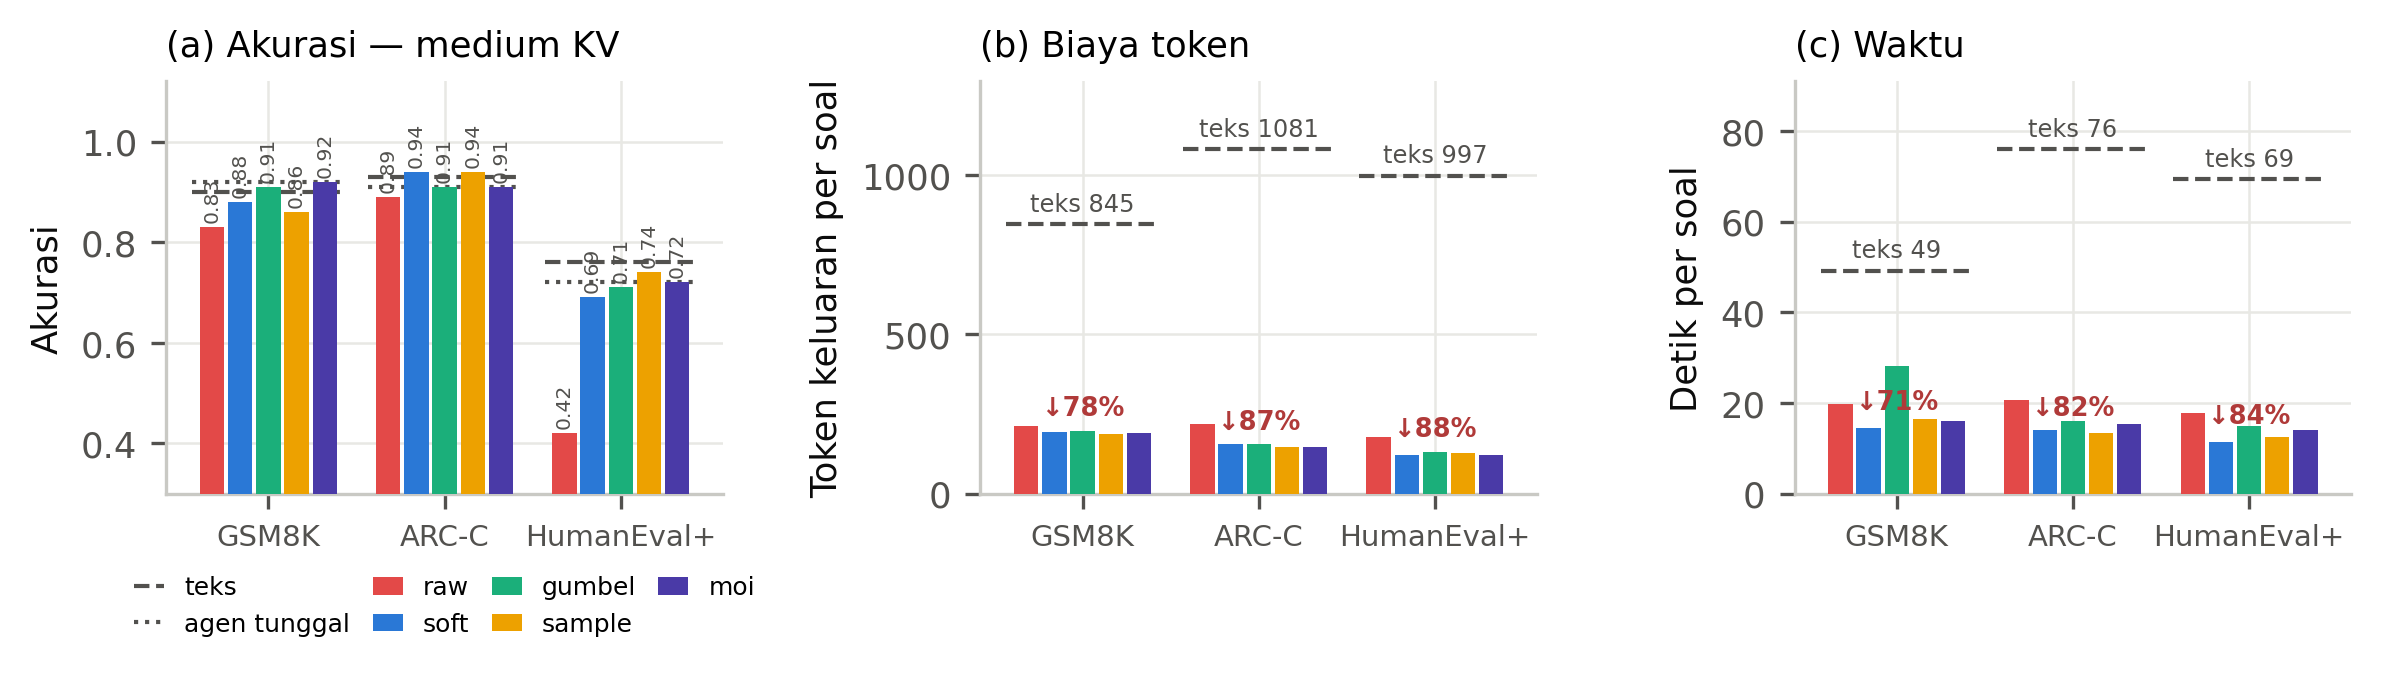
\includegraphics[width=\textwidth]{assets/images/hasil_utama.png}
    \caption{Akurasi, biaya token, dan waktu per soal pada medium KV untuk lima
    persamaan langkah laten. Garis putus-putus menandai medium teks dan garis
    titik-titik menandai agen tunggal. Panel (b) dan (c) mencantumkan
    penghematan sel KV terbaik terhadap medium teks.}
    \label{gbr:hasil-utama}
\end{figure}

Pola akurasi berbeda tajam antar-tugas. Pada GSM8K dan ARC-C, ketujuh perlakuan
berada dalam rentang sempit: 0,83--0,92 pada GSM8K dan 0,89--0,94 pada ARC-C.
Pada HumanEval+, enam perlakuan berada dalam rentang 0,69--0,76, sementara satu
perlakuan --- persamaan langkah laten resmi \code{raw} pada medium KV ---
mencapai 0,42 saja.

\subsection{Uji Berpasangan dan Koreksi Multiplisitas}

Setiap pasangan perlakuan dalam satu tugas diuji dengan uji McNemar eksak pada
hasil benar/salah per soal, disertai selang kepercayaan \textit{bootstrap}
95\% untuk selisih akurasi. Terdapat 21 pasangan per tugas, sehingga seluruhnya
63 pengujian. Karena jumlah pengujian sebesar itu menjamin munculnya temuan
palsu bila dibaca pada taraf nominal, nilai $p$ dikoreksi dengan prosedur Holm
dan Benjamini--Hochberg.

Pada taraf nominal $\alpha = 0{,}05$ terdapat 8 pasangan signifikan. Setelah
koreksi Holm tersisa 6 pasangan, dan koreksi Benjamini--Hochberg memberikan
himpunan yang sama. Dua pasangan yang gugur adalah pasangan GSM8K dengan
$p = 0{,}049$, yaitu tepat di ambang, yang memang tidak bertahan terhadap
koreksi apa pun.

\begin{table}[htbp]
\centering
\caption{Seluruh pasangan yang tetap signifikan setelah koreksi Holm atas 63 uji McNemar eksak. Tak satu pun pasangan pada GSM8K dan ARC-C bertahan; seluruh pasangan yang bertahan berasal dari HumanEval+ dan melibatkan \texttt{raw} pada medium KV.}
\label{tab:uji-signifikan}
\small
\begin{tabular}{llrrrr}
\hline
Tugas & Pasangan & $\Delta$ & SK 95\% & $p$ & $p_{\text{Holm}}$ \\
\hline
HumanEval+ & \texttt{raw/kv} vs \texttt{sample/kv} & -0,320 & [-0,42; -0,22] & $1,9\times 10^{-8}$ & $1,2\times 10^{-6}$ \\
HumanEval+ & \texttt{moi/kv} vs \texttt{raw/kv} & +0,300 & [+0,20; +0,40] & $6,9\times 10^{-8}$ & $4,3\times 10^{-6}$ \\
HumanEval+ & \texttt{raw/baseline} vs \texttt{raw/kv} & +0,300 & [+0,20; +0,40] & $2,3\times 10^{-7}$ & $1,4\times 10^{-5}$ \\
HumanEval+ & \texttt{raw/kv} vs \texttt{raw/text} & -0,340 & [-0,45; -0,22] & $3,1\times 10^{-7}$ & $1,9\times 10^{-5}$ \\
HumanEval+ & \texttt{gumbel/kv} vs \texttt{raw/kv} & +0,290 & [+0,19; +0,40] & $1,1\times 10^{-6}$ & $6,4\times 10^{-5}$ \\
HumanEval+ & \texttt{raw/kv} vs \texttt{soft/kv} & -0,270 & [-0,37; -0,17] & $3,5\times 10^{-6}$ & $2,0\times 10^{-4}$ \\
\hline
\end{tabular}
\end{table}


Tabel~\ref{tab:uji-signifikan} memuat keenam pasangan yang bertahan. Seluruhnya
berasal dari HumanEval+, dan seluruhnya melibatkan \code{raw} pada medium KV.
Tidak ada satu pun pasangan pada GSM8K maupun ARC-C yang bertahan, dan tidak
ada satu pun pasangan antar-anggota keluarga relaksasi yang bertahan pada tugas
mana pun.

\subsection{Homogenitas Kelima Persamaan Langkah Laten}

Uji berpasangan di atas menjawab pertanyaan pasangan-demi-pasangan. Pertanyaan
yang lebih pokok --- apakah kelima persamaan langkah laten berbeda sama sekali
pada suatu tugas --- dijawab dengan uji Cochran $Q$, yaitu uji untuk $k$ sampel
biner berpasangan. Hasilnya disajikan pada Tabel~\ref{tab:cochran}.

\begin{table}[htbp]
\centering
\caption{Uji Cochran $Q$ atas 5 persamaan langkah laten pada medium KV ($n=100$ soal berpasangan).}
\label{tab:cochran}
\begin{tabular}{lrrr}
\hline
Tugas & $Q$ & db & $p$ \\
\hline
GSM8K & 7,40 & 4 & 0,1163 \\
ARC-C & 6,71 & 4 & 0,1518 \\
HumanEval+ & 65,67 & 4 & $<0{,}0001$ \\
\hline
\end{tabular}
\end{table}


Hipotesis nol kesamaan kelima persamaan tidak dapat ditolak pada GSM8K
($p = 0{,}116$) maupun ARC-C ($p = 0{,}152$), tetapi ditolak sangat kuat pada
HumanEval+ ($Q = 65{,}67$; $p < 0{,}0001$). Dengan kata lain, pada dua tugas
penalaran umum pilihan persamaan langkah laten tidak dapat dibedakan dari
derau, sedangkan pada tugas pembangkitan kode ia menentukan.

\subsection{Kontras Keluarga Relaksasi terhadap Ridge $W_a$}

Karena hipotesis penelitian menyangkut keanggotaan pada keluarga relaksasi
diskret dan bukan keunggulan satu varian, kontras utama dihitung antara rerata
keempat anggota keluarga (\code{soft}, \code{gumbel}, \code{sample},
\code{moi}) dan persamaan resmi \code{raw}, pada tingkat soal. Hasilnya
disajikan pada Tabel~\ref{tab:kontras}.

\begin{table}[htbp]
\centering
\caption{Kontras akurasi antara rerata keluarga relaksasi diskret dan ridge $W_a$ (\texttt{raw}) pada medium KV, dengan selang kepercayaan \textit{bootstrap} 95\%.}
\label{tab:kontras}
\begin{tabular}{lrrl}
\hline
Tugas & \texttt{raw} & Keluarga & $\Delta$ dan SK 95\% \\
\hline
GSM8K & 0,83 & 0,892 & $+0{,}062$ \quad [$-0{,}005$; $+0{,}135$] \\
ARC-C & 0,89 & 0,925 & $+0{,}035$ \quad [$-0{,}003$; $+0{,}080$] \\
HumanEval+ & 0,42 & 0,715 & $+0{,}295$ \quad [$+0{,}205$; $+0{,}388$] \\
\hline
\end{tabular}
\end{table}


Pada GSM8K dan ARC-C, selang kepercayaan memuat nol, sehingga keunggulan
keluarga relaksasi tidak dapat dinyatakan. Pada HumanEval+, selisihnya
$+0{,}295$ dengan selang kepercayaan yang jauh dari nol.

\section{Disosiasi menurut Tuntutan Presisi Simbolik}
\label{sec:disosiasi}

Ketiga hasil di atas menunjuk pada satu kesimpulan yang sama: kerugian akibat
memakai persamaan langkah laten resmi tidak seragam antar-tugas, melainkan
terkonsentrasi pada tugas yang menuntut ketepatan simbol. Untuk mengujinya
secara langsung, selisih $\Delta_t$ pada Tabel~\ref{tab:kontras} dibandingkan
antar-tugas. Karena ketiga tugas memakai soal yang berbeda, perbandingan
antar-tugas bersifat tak-berpasangan dan selang kepercayaan selisihnya dihitung
dengan \textit{bootstrap} independen per tugas.

\begin{table}[htbp]
\centering
\caption{Perbandingan besar kerusakan $\Delta$ antar-tugas. Tugas dengan kerusakan lebih besar disebut lebih dulu pada tiap baris.}
\label{tab:disosiasi}
\begin{tabular}{lrll}
\hline
Pasangan tugas & $\Delta\Delta$ & SK 95\% & $p$ \\
\hline
GSM8K vs ARC-C & $+0{,}027$ & [$-0{,}055$; $+0{,}113$] & 0,5422 \\
HumanEval+ vs ARC-C & $+0{,}260$ & [$+0{,}157$; $+0{,}360$] & $<0{,}0001$ \\
HumanEval+ vs GSM8K & $+0{,}232$ & [$+0{,}115$; $+0{,}347$] & 0,0002 \\
\hline
\end{tabular}
\end{table}


Tabel~\ref{tab:disosiasi} dan Gambar~\ref{gbr:disosiasi} menunjukkan bahwa
kerusakan pada HumanEval+ berbeda secara meyakinkan dari kerusakan pada kedua
tugas lain, sedangkan GSM8K dan ARC-C tidak dapat dibedakan satu sama lain.

\begin{figure}[htbp]
    \centering
    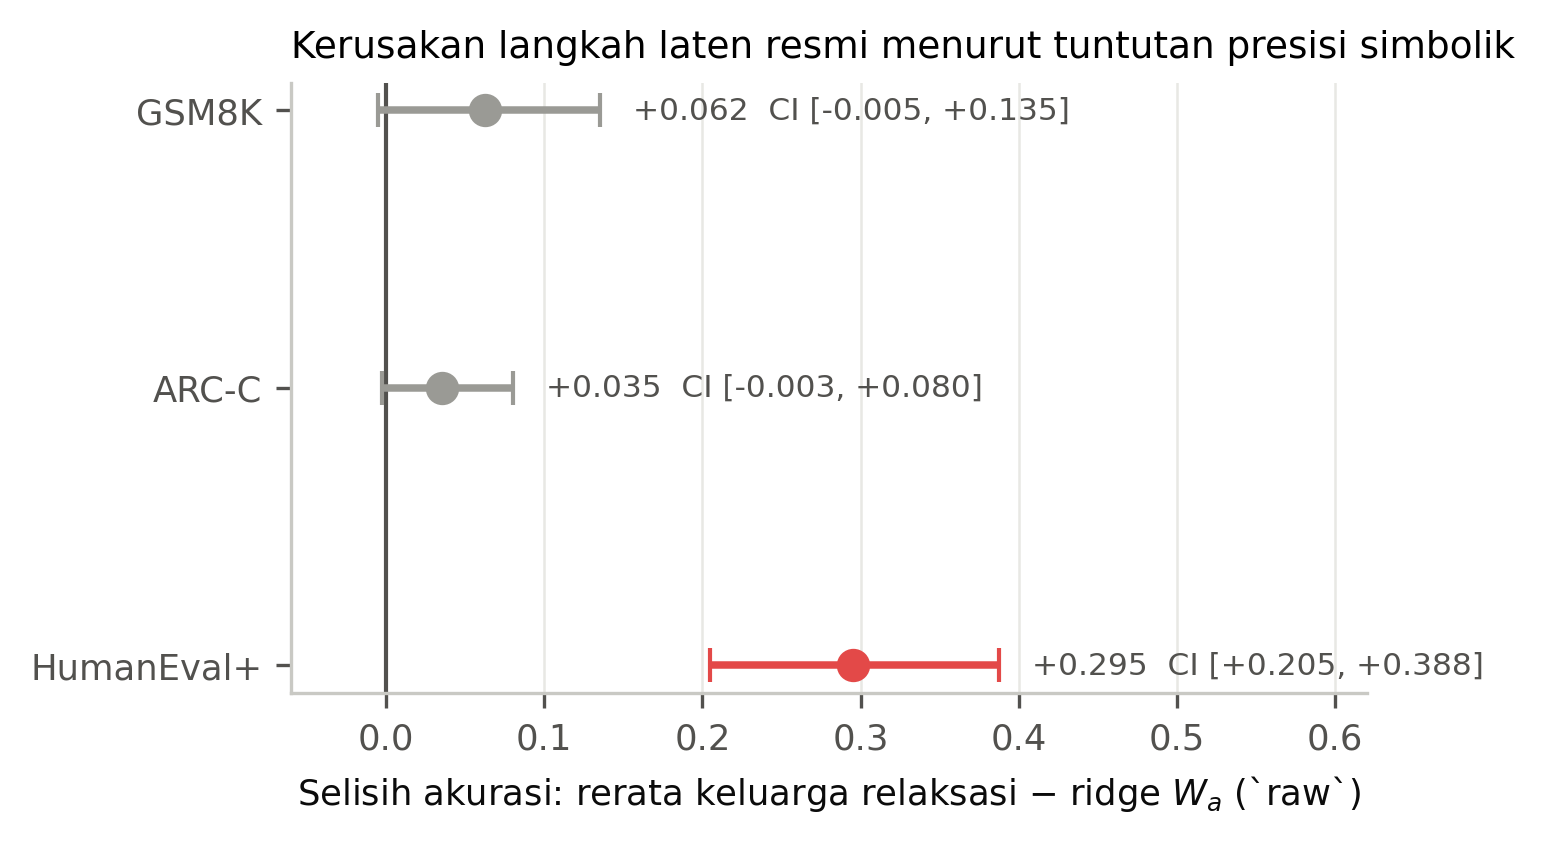
\includegraphics[width=0.85\textwidth]{assets/images/disosiasi.png}
    \caption{Selisih akurasi antara rerata keluarga relaksasi diskret dan ridge
    $W_a$ pada ketiga tugas, dengan selang kepercayaan \textit{bootstrap} 95\%.}
    \label{gbr:disosiasi}
\end{figure}

Temuan ini mengonfirmasi sebagian hipotesis H2 pada Bab~III. Bagian yang
terkonfirmasi adalah disosiasi itu sendiri: tugas dengan tuntutan presisi
simbolik tertinggi --- pembangkitan kode yang harus lolos eksekusi ---
mengalami kerusakan yang jauh lebih besar daripada tugas berjawaban pendek.
Bagian yang tidak terkonfirmasi adalah urutan tiga tingkat yang diramalkan:
GSM8K dan ARC-C tidak berbeda satu sama lain ($p = 0{,}542$), sehingga yang
didukung data adalah pembedaan dua tingkat, bukan tiga.

Perlu dicatat bahwa urutan ini diramalkan pada dokumen rancangan eksperimen
sebelum sel \textit{benchmark} dijalankan, berdasarkan pengukuran kapasitas
kanal simbolik yang dibahas pada \ref{sec:mekanisme}. Statusnya karena itu
adalah ramalan yang kemudian diuji, bukan penjelasan yang disusun setelah
melihat angka.

Satu pembacaan alternatif perlu ditutup di sini. Kerusakan pada HumanEval+
dapat saja berasal dari medium KV, bukan dari persamaan langkah laten. Namun
pembacaan itu tidak sejalan dengan data: pada tugas yang sama, empat perlakuan
lain yang juga memakai medium KV mencapai 0,69--0,74, yakni setara dengan agen
tunggal (0,72) dan medium teks (0,76). Yang membedakan sel yang runtuh dari
keenam sel lainnya bukan mediumnya, melainkan persamaan langkah latennya.

\section{Efisiensi Medium Laten}
\label{sec:efisiensi}

Klaim utama kerangka LatentMAS \citep{latentmas} bersifat efisiensi: kolaborasi
laten dilaporkan menurunkan pemakaian token keluaran 70,8\%--83,7\% dan
mempercepat inferensi $4\times$--$4{,}3\times$ dibanding kolaborasi berbasis
teks. Karena penelitian ini menjalankan kedua medium pada pipeline yang sama,
klaim tersebut dapat diuji ulang secara langsung.

\begin{table}[htbp]
\centering
\caption{Efisiensi medium KV relatif terhadap medium teks, per persamaan langkah laten. Penghematan token dihitung atas token keluaran per soal; percepatan atas waktu dinding per soal. Kolom akurasi diulang dari Tabel~\ref{tab:hasil-bench} supaya biaya dan mutu terbaca pada satu baris.}
\label{tab:efisiensi}
\small
\begin{tabular}{llrrr}
\hline
Tugas & Langkah laten & Akurasi & Penghematan token & Percepatan \\
\hline
ARC-C & \texttt{raw} & 0,89 & 79,7\% & $\times3,7$ \\
ARC-C & \texttt{soft} & 0,94 & 85,7\% & $\times5,4$ \\
ARC-C & \texttt{gumbel} & 0,91 & 85,7\% & $\times4,8$ \\
ARC-C & \texttt{sample} & 0,94 & 86,5\% & $\times5,7$ \\
ARC-C & \texttt{moi} & 0,91 & 86,6\% & $\times5,0$ \\
\hline
GSM8K & \texttt{raw} & 0,83 & 75,0\% & $\times2,5$ \\
GSM8K & \texttt{soft} & 0,88 & 77,2\% & $\times3,4$ \\
GSM8K & \texttt{gumbel} & 0,91 & 76,7\% & $\times1,8$ \\
GSM8K & \texttt{sample} & 0,86 & 77,8\% & $\times3,0$ \\
GSM8K & \texttt{moi} & 0,92 & 77,5\% & $\times3,1$ \\
\hline
HumanEval+ & \texttt{raw} & 0,42 & 82,3\% & $\times3,9$ \\
HumanEval+ & \texttt{soft} & 0,69 & 87,8\% & $\times6,1$ \\
HumanEval+ & \texttt{gumbel} & 0,71 & 86,9\% & $\times4,7$ \\
HumanEval+ & \texttt{sample} & 0,74 & 87,4\% & $\times5,6$ \\
HumanEval+ & \texttt{moi} & 0,72 & 87,8\% & $\times4,9$ \\
\hline
\end{tabular}
\end{table}


Tabel~\ref{tab:efisiensi} menunjukkan penghematan token keluaran 75,0\%--87,8\%
dan percepatan $\times1{,}8$--$\times6{,}1$ terhadap medium teks. Rentang
penghematan token memuat dan sedikit melampaui rentang yang dilaporkan paper
asal, sehingga klaim efisiensi kerangka tersebut terreplikasi pada perangkat
keras, model, dan implementasi yang berbeda.

Mekanisme penghematannya terbaca langsung dari jumlah panggilan model: pada
medium teks setiap soal memicu 400 panggilan berkeluaran teks untuk 100 soal
(empat agen per soal), sedangkan pada medium KV hanya 100 panggilan, karena
tiga agen perantara menyerahkan pekerjaan lewat KV-\textit{cache} tanpa pernah
memverbalkan penalarannya.

Gambar~\ref{gbr:akurasi-token} menempatkan akurasi dan biaya token pada satu
bidang. Pada GSM8K dan ARC-C, sel KV dengan persamaan dari keluarga relaksasi
menempati kuadran yang diinginkan: akurasi setara medium teks dengan biaya
token sekitar seperlima hingga sepertujuh. Pada HumanEval+, sel \code{raw}
terpisah jelas dari kelompok tersebut.

\begin{figure}[htbp]
    \centering
    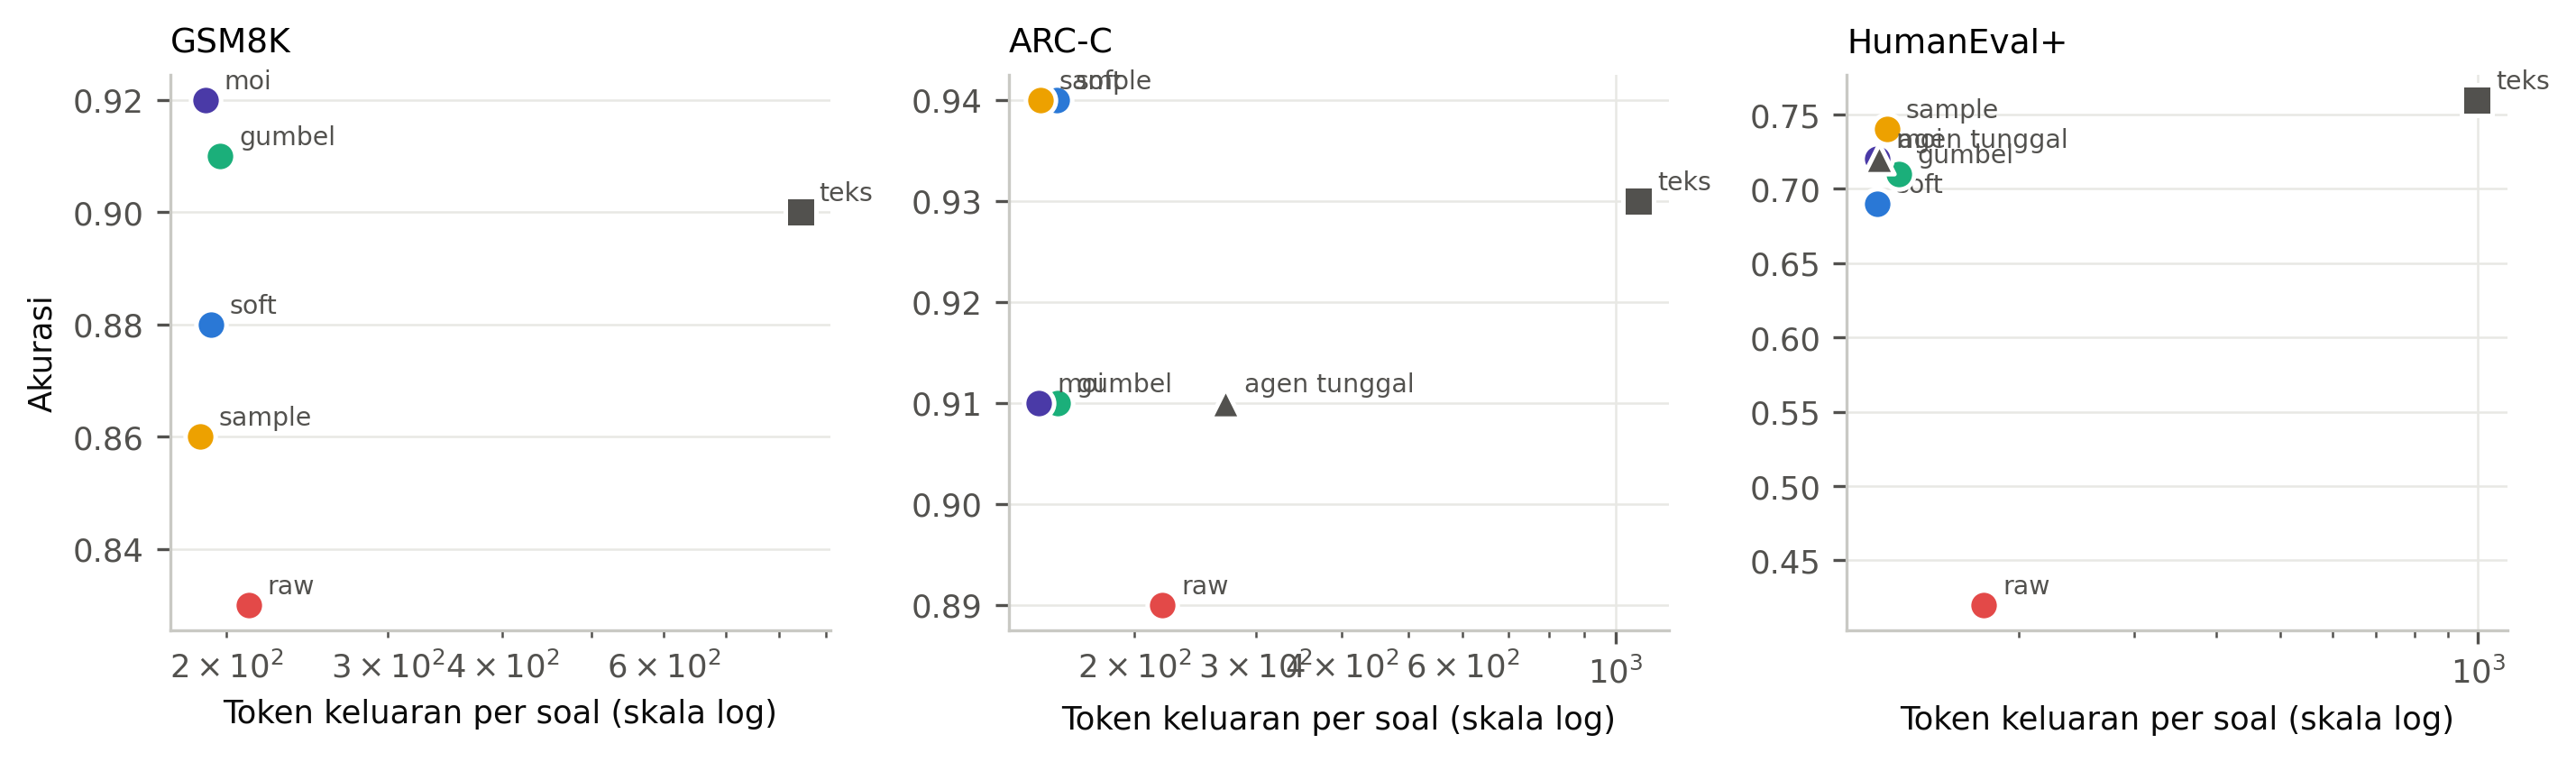
\includegraphics[width=\textwidth]{assets/images/akurasi_vs_token.png}
    \caption{Akurasi terhadap biaya token keluaran per soal (skala logaritmik).
    Titik berwarna adalah medium KV dengan lima persamaan langkah laten;
    penanda kelabu adalah medium teks dan agen tunggal.}
    \label{gbr:akurasi-token}
\end{figure}

Perlu dinyatakan bahwa keunggulan biaya ini tidak disertai keunggulan akurasi.
Terhadap medium teks, akurasi sel KV terbaik lebih tinggi pada ARC-C
(0,94 vs 0,93) dan GSM8K (0,92 vs 0,90), tetapi lebih rendah pada HumanEval+
(0,74 vs 0,76); tak satu pun selisih tersebut signifikan. Rumusan yang didukung
data adalah kesetaraan akurasi pada biaya yang jauh lebih rendah, bukan
keunggulan akurasi.

\section{Fidelitas Simbolik Keluaran}
\label{sec:fidelitas}

Akurasi menggabungkan dua hal yang perlu dipisahkan: apakah jawaban benar, dan
apakah keluaran berbentuk sah. Keduanya dilaporkan terpisah.

Tingkat keluaran berformat sah (\textit{format rate}) berada pada 0,96--1,00 di
seluruh 21 sel utama, sehingga tidak ada perlakuan yang gagal secara
struktural. Nilai terendah dijumpai pada \code{soft} di HumanEval+ (0,96) dan
\code{sample} di GSM8K (0,97).

Ukuran kedua lebih informatif. Karena seluruh tugas berbahasa Inggris,
kemunculan aksara Tionghoa di dalam jawaban menandai token dari ruang bahasa
lain yang menyusup ke keluaran --- bentuk kerusakan identitas token yang dapat
diperiksa secara langsung. Tabel~\ref{tab:korupsi} melaporkan cacahnya.

\begin{table}[htbp]
\centering
\caption{Jumlah jawaban yang memuat aksara Tionghoa pada tugas berbahasa Inggris, dari 100 jawaban per sel.}
\label{tab:korupsi}
\small
\begin{tabular}{lrrrrrrr}
\hline
Tugas & Tunggal & Teks & \texttt{raw} & \texttt{soft} & \texttt{gumbel} & \texttt{sample} & \texttt{moi} \\
\hline
GSM8K & --- & 0 & 2 & 0 & 0 & 0 & 1 \\
ARC-C & 0 & 0 & 3 & 1 & 1 & 0 & 0 \\
HumanEval+ & 0 & 0 & 1 & 0 & 0 & 0 & 0 \\
\hline
Jumlah & 0 & 0 & 6 & 1 & 1 & 0 & 1 \\
\hline
\end{tabular}
\end{table}


Cacah keseluruhan kecil dan tidak memungkinkan pengujian formal, tetapi arahnya
konsisten: enam dari sembilan kejadian berasal dari \code{raw}, sedangkan
medium teks dan agen tunggal --- keduanya tanpa langkah laten --- tidak pernah
mengalaminya. Pada satu jawaban sel \code{raw} ARC-C, frasa \code{"the effects
of a hypoxic event."} tercatat dengan kata terakhirnya tergantikan oleh padanan
dua-aksara Tionghoa, yaitu substitusi token di tengah kalimat yang
mempertahankan makna tetapi merusak bentuk keluaran.

Contoh yang paling menjelaskan berasal dari HumanEval+, tempat kerusakannya
berakibat fatal karena keluarannya harus dieksekusi. Salah satu jawaban sel
\code{raw} memuat penggalan \code{'No'\ \ \#Count.digits.in} yang diikuti dua
aksara Tionghoa. Dua bentuk kerusakan tampak sekaligus pada satu baris: spasi
antar-kata tergantikan tanda titik, dan token dari ruang bahasa lain menyusup
di tengah pengenal. Pada tugas berjawaban pendek kerusakan semacam itu masih
dapat dipulihkan oleh agen berikutnya; pada kode, satu pengenal yang salah
membuat seluruh program gagal dieksekusi. Inilah bentuk konkret dari disosiasi
yang diukur pada \ref{sec:disosiasi}. Daftar lengkap cuplikan yang terekam
disajikan pada Lampiran~\ref{lamp:transkrip}.

Pola yang sama muncul kembali, dalam bentuk yang jauh lebih parah, pada lengan
faktor (\ref{sec:faktor}).

\section{Bukti Mekanisme}
\label{sec:mekanisme}

Bagian ini menghubungkan pola akurasi di atas dengan sifat geometris persamaan
langkah laten yang diuraikan pada Bab~III.

\begin{table}[htbp]
\centering
\caption{Geometri vektor langkah laten pada Qwen3-8B. Kolom terakhir adalah kosinus terhadap baris matriks embedding masukan yang paling dekat; nilai $1$ berarti vektor tepat berimpit dengan embedding sebuah token.}
\label{tab:geometri}
\small
\begin{tabular}{lccc}
\hline
Langkah laten & Bentuk & Anggota ($\star$) & $\max_i \cos(\Phi(h), W_{\text{in}}[i])$ \\
\hline
\texttt{raw} & $\rho\,hM/\lVert hM\rVert$ & tidak & 0,312 [0,16; 0,38] \\
\texttt{soft} & $w = p$ & ya & 0,927 [0,78; 1,00] \\
\texttt{gumbel} & $w = \mathrm{softmax}((\ell+g)/T)$ & ya & 0,985 [0,86; 1,00] \\
\texttt{sample} & $w = e_y$ & ya & 1,000 [1,00; 1,00] \\
\hline
\multicolumn{4}{l}{\footnotesize $\lVert M-I\rVert_F/\lVert I\rVert_F = 1,04$;\quad $\cos(h, hM)$ rerata $= 0,0112$;\quad $\cos(W_{\text{in}}[i], W_{\text{out}}[i])$ rerata $= 0,0041$.} \\
\end{tabular}
\end{table}


Tabel~\ref{tab:geometri} melaporkan kosinus antara vektor langkah laten dan
baris matriks embedding masukan yang paling dekat dengannya. Anggota keluarga
relaksasi menghasilkan vektor yang sangat dekat dengan embedding token nyata:
0,927 untuk \code{soft}, 0,985 untuk \code{gumbel}, dan tepat 1,000 untuk
\code{sample} --- nilai terakhir memang harus demikian, karena bobot
campurannya adalah vektor satuan sehingga hasilnya persis satu baris embedding
yang diskalakan. Sebaliknya, \code{raw} menghasilkan 0,312, yaitu vektor yang
tidak menyerupai embedding token mana pun.

\begin{figure}[htbp]
    \centering
    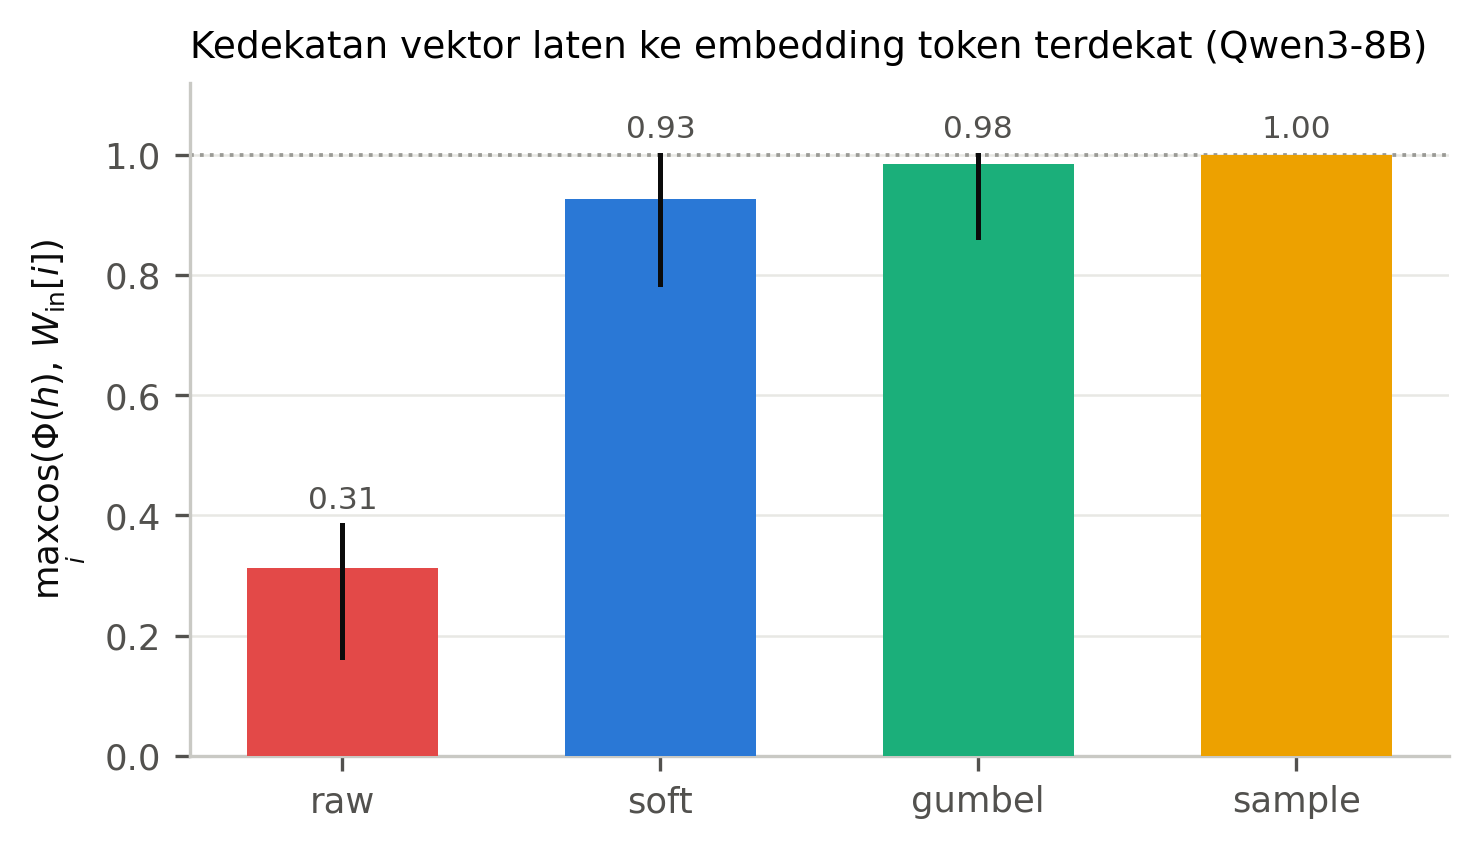
\includegraphics[width=0.85\textwidth]{assets/images/geometri_langkah_laten.png}
    \caption{Kosinus terhadap embedding token terdekat untuk empat persamaan
    langkah laten pada Qwen3-8B. Batang menunjukkan rerata atas sepuluh langkah
    laten; garis vertikal menunjukkan rentang minimum--maksimum.}
    \label{gbr:geometri}
\end{figure}

Tiga besaran pendukung pada catatan kaki Tabel~\ref{tab:geometri} melengkapi
gambarannya. Simpangan relatif matriks realignment terhadap identitas adalah
1,04, sehingga $M$ benar-benar memutar vektor dan bukan sekadar
menskalakannya. Kosinus antara \textit{hidden state} dan hasil pemetaannya
hanya 0,0112, yaitu nyaris tegak lurus. Kosinus antara baris embedding masukan
dan baris embedding keluaran yang bersesuaian hanya 0,0041, yang menjelaskan
mengapa pemetaan tersebut harus memutar sejauh itu.

Perlu ditekankan bahwa keadaan ini bergantung pada model. Pada Qwen3-4B kedua
matriks embedding berbagi bobot (\textit{tied embeddings}) sehingga $M$
mendekati identitas dan persamaan \code{raw} praktis tidak melakukan apa pun.
Pada Qwen3-8B keduanya terpisah. Penelitian ini dipatok pada Qwen3-8B justru
karena pada model dengan embedding terikat tidak ada yang dapat diperbaiki, dan
seluruh perbandingan menjadi hampa.

Bukti kedua berasal dari pengukuran kapasitas kanal laten yang dilakukan
sebelum lengan \textit{benchmark} dijalankan. Pada kanal laten murni yang
membawa muatan simbolik berupa nama fungsi, persamaan \code{raw} memberikan
\textit{recall} 0,000 --- nol mutlak, bukan sekadar rendah --- sedangkan
keempat anggota keluarga relaksasi berada pada 0,34--0,38 dengan $m=10$ dan
0,72--0,87 dengan $m=40$. Perbedaan antar-anggota keluarga tidak signifikan
pada $n=20$.

Ketiga potongan bukti tersebut menyusun satu penjelasan yang runtut. Persamaan
resmi menempatkan vektor laten di luar lambung konveks embedding, tempat
perilaku model tidak terdefinisi. Akibatnya identitas token diskret rusak, yang
terlihat sebagai \textit{recall} nol pada kanal simbolik dan sebagai aksara
asing yang menyusup ke jawaban. Tugas yang toleran terhadap lintasan penalaran
yang kabur --- soal cerita berjawaban satu bilangan, soal pilihan berjawaban
satu huruf --- dapat pulih dari kerusakan itu; tugas yang menuntut setiap
pengenal ditulis persis tidak dapat.

Penjelasan ini juga menunjukkan letak kekeliruan penafsiran yang mudah terjadi.
Teorema pemeliharaan informasi pada kerangka LatentMAS menyangkut
\textit{pengangkutan} KV antar-agen, dan tidak ada pada data ini yang
membantahnya. Yang bermasalah adalah \textit{pembangkitan} vektor laten oleh
persamaan langkah laten. Kedua hal itu terpisah, dan hanya yang kedua yang
diperbaiki oleh keluarga relaksasi diskret.

\section{Lengan Faktor Simbolik}
\label{sec:faktor}

Sebagaimana ditetapkan pada Bab~III, lengan faktor simbolik diperlakukan
sebagai kondisi pelengkap, bukan sebagai sel eksperimen penuh. Fungsinya adalah
menguji kanal yang sama pada muatan yang seluruhnya berupa simbol, yaitu
ekspresi DSL yang harus dapat diurai dan dievaluasi. Bagian ini melaporkan tiga
hal: keandalan keluaran agen penyusun ekspresi, mutu ekspresi yang dihasilkan,
dan beberapa faktor konkret sebagai bukti kualitatif.

\subsection{Artefak Medium Gabungan dan Pemulihannya}

Pemeriksaan awal menemukan bahwa pada medium gabungan KV dan teks, keluaran
agen penyusun tidak dapat diurai sama sekali sehingga sel-sel tersebut
tercatat menghasilkan nol ekspresi. Pembacaan keluaran mentahnya menunjukkan
bahwa penyebabnya bukan kegagalan model: keluarannya kehilangan tepat prefiks
pembuka objek JSON, sedangkan sisanya utuh dan sah. Kehilangan tersebut terjadi
pada seluruh panggilan di empat dari lima sel medium gabungan, yaitu pola yang
sistematis dan bukan ragam acak.

Karena bentuk kehilangannya tetap, prefiks tersebut dapat dikembalikan secara
deterministik. Aturan pemulihan diterapkan seragam ke seluruh sel, dan secara
empiris tidak pernah aktif pada sel yang keluarannya sudah normal: dari 77
panggilan pada medium teks dan medium KV, tak satu pun memerlukan pemulihan.
Sifat itu penting karena berarti aturan tersebut tidak dapat mengubah sel yang
sehat, sehingga penerapannya tidak menguntungkan atau merugikan satu metode
pun. Setelah pemulihan, keempat sel tersebut menghasilkan 30--37 ekspresi unik,
dengan 16--29 di antaranya lolos \textit{gate} mutu.

Penyebab teknis kehilangan prefiks tersebut tidak ditelusuri sampai tuntas dan
dicatat sebagai keterbatasan. Konsekuensi metodologisnya dinyatakan di sini:
angka medium gabungan pada lengan faktor tidak dipakai untuk membandingkan
medium, melainkan hanya untuk menunjukkan bahwa keluaran modelnya memang
ekspresi yang sah.

\subsection{Keandalan Keluaran Agen Penyusun}

Ukuran yang paling langsung pada lengan ini tidak memerlukan data pasar sama
sekali, yaitu apakah keluaran agen penyusun dapat diurai menjadi objek yang
sah. Ukuran tersebut merupakan padanan \textit{format rate} pada lengan
\textit{benchmark}, tetapi dengan tuntutan yang lebih ketat karena keluarannya
harus memuat ekspresi DSL yang lengkap.

\begin{table}[htbp]
\centering
\caption{Keluaran agen \textit{construct} pada lengan faktor simbolik. Kolom \textsc{Gagal} adalah panggilan yang keluarannya tidak dapat diurai menjadi objek JSON yang sah; kolom \textsc{Pulih} adalah panggilan yang hanya kehilangan prefiks pembuka objek dan dapat dipulihkan secara deterministik.}
\label{tab:faktor-parsing}
\small
\begin{tabular}{llrrrrr}
\hline
Medium & Metode & Panggilan & Utuh & Pulih & Gagal & Gagal (\%) \\
\hline
teks & \texttt{raw} & 12 & 12 & 0 & 0 & 0 \\
kv & \texttt{raw} & 18 & 4 & 0 & 14 & 78 \\
kv & \texttt{soft} & 7 & 7 & 0 & 0 & 0 \\
kv & \texttt{gumbel} & 16 & 10 & 0 & 6 & 38 \\
kv & \texttt{sample} & 10 & 6 & 0 & 4 & 40 \\
kv & \texttt{moi} & 14 & 10 & 0 & 4 & 29 \\
kv+teks & \texttt{raw} & 15 & 5 & 0 & 10 & 67 \\
kv+teks & \texttt{soft} & 12 & 0 & 12 & 0 & 0 \\
kv+teks & \texttt{gumbel} & 12 & 0 & 12 & 0 & 0 \\
kv+teks & \texttt{sample} & 12 & 0 & 12 & 0 & 0 \\
kv+teks & \texttt{moi} & 18 & 0 & 14 & 4 & 22 \\
\hline
\end{tabular}
\end{table}


Tabel~\ref{tab:faktor-parsing} menunjukkan pola yang sejajar dengan temuan pada
HumanEval+. Medium teks dan mode \code{soft} pada medium KV tidak pernah gagal.
Ketiga anggota keluarga relaksasi lainnya gagal pada 29\%--40\% panggilan.
Persamaan resmi \code{raw} gagal pada 14 dari 18 panggilan, yaitu 78\%.

Kegagalan pada \code{raw} juga berbeda secara kualitatif. Keluarannya bukan
sekadar terpotong, melainkan rusak di tingkat kata: kunci JSON tertulis sebagai
\code{"f actor"} dan \code{"hypo"}, sementara kalimat hipotesisnya kehilangan
spasi dan mengulang suku kata, seperti pada penggalan
\code{"abnormallylyhigh-volumeolumedayssin small-capstocksocks"}. Bentuk
kerusakan ini identik dengan yang terekam pada lengan \textit{benchmark}
(\ref{sec:fidelitas}), yakni hilangnya identitas token pada tingkat sub-kata.
Pada tugas berjawaban pendek kerusakan tersebut jarang berakibat fatal; pada
ekspresi DSL, satu nama fungsi yang rusak membuat seluruh ekspresi tidak dapat
diurai.

\subsection{Mutu Ekspresi yang Dihasilkan}

\begin{table}[htbp]
\centering
\caption{Korpus ekspresi yang benar-benar diserahkan sistem ujung-ke-ujung pada medium \texttt{text} dan \texttt{kv} (enam jalannya per sel). Ekspresi disebut hidup bila RankIC-nya terdefinisi dan skornya tidak konstan.}
\label{tab:faktor-korpus}
\small
\begin{tabular}{llrrrr}
\hline
Medium & Metode & Ekspresi & Dapat dievaluasi & $\overline{|\text{RankIC}|}$ & $|t|\ge1{,}96$ \\
\hline
teks & \texttt{raw} & 36 & 20 & 0,0184 & 12 \\
kv & \texttt{raw} & 11 & 3 & 0,0050 & 2 \\
kv & \texttt{soft} & 33 & 25 & 0,0173 & 17 \\
kv & \texttt{gumbel} & 30 & 26 & 0,0162 & 14 \\
kv & \texttt{sample} & 22 & 21 & 0,0185 & 16 \\
kv & \texttt{moi} & 28 & 22 & 0,0171 & 12 \\
\hline
\end{tabular}
\end{table}


Tabel~\ref{tab:faktor-korpus} melaporkan korpus yang benar-benar diserahkan
sistem ujung-ke-ujung pada medium teks dan medium KV. Perbedaan
produktivitasnya besar: \code{raw} menghasilkan 11 ekspresi dengan 3 di
antaranya dapat dievaluasi, sedangkan keempat anggota keluarga relaksasi
menghasilkan 22--33 ekspresi dengan 21--26 dapat dievaluasi. Dengan kata lain,
pada jumlah jalan yang sama, persamaan resmi menghasilkan sekitar sepertujuh
ekspresi yang berguna dibanding alternatifnya.

Rerata $|\text{RankIC}|$ ekspresi yang hidup berada pada 0,0162--0,0185 untuk
medium teks dan keempat anggota keluarga relaksasi, sedangkan \code{raw} hanya
mencapai 0,0050. Perlu ditekankan bahwa angka \code{raw} dihitung dari tiga
ekspresi saja, sehingga selisih tersebut tidak layak diuji secara formal dan
tidak diklaim signifikan. Yang didukung data adalah pernyataan yang lebih
sederhana dan lebih kuat: pada lengan ini persamaan resmi sebagian besar gagal
menghasilkan ekspresi yang dapat dinilai sama sekali.

\subsection{Beberapa Faktor Konkret}

\begin{table}[htbp]
\centering
\caption{Faktor dengan statistik-$t$ RankIC terbesar pada tiap sel medium yang menghasilkan ekspresi hidup, beserta metrik \textit{backtest} portofolio desil \textit{long--short}. Angka \textit{backtest} tidak boleh dibaca sebagai ramalan keuntungan; lihat batas berlaku.}
\label{tab:kartu-faktor}
\small
\begin{tabular}{llrrrrr}
\hline
Sel & Ekspresi & RankIC & $t$ & ARR & Sharpe & MDD \\
\hline
teks/\texttt{raw} & \texttt{\scriptsize RANK(TS\_ARGMAX(\$return, 20 ... (\$volume, 30)} & +0,0383 & +6,59 & +0,298 & +2,30 & -0,087 \\
kv/\texttt{gumbel} & \texttt{\scriptsize TS\_QUANTILE(\$volume, 20, 0 ... ume, 20, 0.1)} & -0,0394 & -5,80 & -0,361 & -2,45 & -0,373 \\
kv/\texttt{moi} & \texttt{\scriptsize INV(LOG(SUMAC(\$volume, 10) ...  \$return, 30)} & -0,0346 & -5,36 & -0,202 & -1,60 & -0,223 \\
kv/\texttt{sample} & \texttt{\scriptsize TS\_MAD(TS\_SUM(\$volume, 5), ... eturn, 5), 5)} & -0,0194 & -5,19 & -0,209 & -2,49 & -0,262 \\
kv/\texttt{soft} & \texttt{\scriptsize TS\_QUANTILE(\$volume, 20, 0 ... E(\$return, 1)} & -0,0310 & -5,66 & -0,269 & -2,68 & -0,287 \\
\hline
\end{tabular}
\end{table}


Tabel~\ref{tab:kartu-faktor} menyajikan satu faktor dengan statistik-$t$
terbesar dari setiap sel yang menghasilkan ekspresi hidup, lengkap dengan
metrik portofolio desil \textit{long--short}. Faktor-faktor tersebut memiliki
$|t|$ antara 5 dan 7, yang menunjukkan daya prediksi yang berbeda dari nol pada
jendela yang diuji.

Tiga catatan pembacaan perlu disertakan. Pertama, tanda RankIC tidak menentukan
kegunaan sebuah faktor, karena faktor berkorelasi negatif dapat dipakai dengan
membalik arah posisi; nilai ARR dan Sharpe yang negatif pada tabel merupakan
konsekuensi langsung dari konvensi arah tersebut, bukan penanda faktor yang
buruk. Kedua, angka \textit{backtest} berasal dari simulasi kasar tanpa
\textit{slippage}, tanpa batas likuiditas, dan dengan penyeimbangan ulang
harian penuh, sehingga tidak boleh dibaca sebagai ramalan keuntungan. Ketiga,
seluruh angka dihitung pada jendela yang sama untuk semua metode, sehingga
perbandingan antar-metode tetap sah meskipun angka mutlaknya terbatas.

Ekspresi hasil pemulihan pada medium gabungan juga dinilai untuk sebagian kecil
sampel guna memastikan bahwa keluarannya memang ekspresi yang berfungsi.
Sebagai contoh, ekspresi \code{RANK(TS\_ZSCORE(TS\_ARGMAX(\$volume, 5), 20))}
dari sel \code{moi} memberikan RankIC $0{,}0147$ dengan $t = 4{,}49$, sedangkan
\code{RANK(\$return) / TS\_MAD(\$volume, 15)} dari sel \code{sample}
memberikan RankIC $0{,}0310$ dengan $t = 4{,}21$. Keduanya menunjukkan bahwa
keluaran yang semula tercatat sebagai kegagalan total sebenarnya memuat
ekspresi yang sah dan bermuatan sinyal.

\subsection{Kedudukan terhadap Hipotesis H2}

Hipotesis H2 pada Bab~III meramalkan bahwa kerusakan akibat persamaan resmi
meningkat seiring tuntutan presisi simbolik tugas, dengan domain faktor
simbolik berada pada ujung paling menuntut. Hasil pada lengan ini sejalan
dengan ramalan tersebut: pada tugas berjawaban pendek selisihnya tidak
signifikan, pada pembangkitan kode selisihnya 0,295, dan pada pembangkitan
ekspresi DSL persamaan resmi gagal pada 78\% panggilan sehingga sebagian besar
keluarannya tidak sampai pada tahap penilaian.

Perbandingan pada lengan ini bersifat deskriptif dan tidak diuji secara formal,
karena jumlah jalan per sel kecil dan satuan pengamatannya berbeda dari lengan
\textit{benchmark}. Karena itu lengan faktor dilaporkan sebagai bukti
pendukung yang arahnya konsisten, bukan sebagai pengujian mandiri terhadap H2.

\section{Batas Berlaku dan Ancaman Validitas}
\label{sec:batas}

Sejumlah batas perlu dinyatakan agar kesimpulan bab ini tidak dibaca melampaui
dukungan datanya.

\begin{enumerate}
    \item Satu \textit{backbone}. Seluruh angka diperoleh pada
          Qwen3-8B. Sebagaimana dibahas pada \ref{sec:mekanisme}, hasilnya
          bergantung pada apakah kedua matriks embedding model terikat atau
          tidak, sehingga generalisasi lintas ukuran maupun lintas keluarga
          model tidak diuji dan tidak diklaim.
    \item Satu \textit{seed}. Setiap sel dijalankan satu kali. Ragam
          antar-\textit{seed} karena itu tidak terukur, dan selang kepercayaan
          yang dilaporkan hanya mencakup ragam antar-soal.
    \item Subsampel 100 soal. Angka akurasi tidak sebanding langsung
          dengan angka yang dilaporkan atas himpunan uji penuh.
    \item Medium \textit{kv\_and\_text} tidak diuji. Sebagaimana
          dinyatakan pada \ref{sec:cakupan}, medium tersebut hanya berjalan
          pada lima soal per sel sebagai pemasok lampiran.
    \item Urutan tiga tingkat tidak terkonfirmasi. Data mendukung
          pembedaan dua tingkat (kode versus selebihnya), bukan urutan
          GSM8K $<$ ARC-C $<$ HumanEval+ yang diramalkan.
    \item \textit{Backtest} bersifat kasar. Sebagaimana dinyatakan
          pada \ref{sec:faktor}, simulasi portofolio berjalan tanpa
          \textit{slippage}, tanpa batas likuiditas, dan tanpa aturan suspensi
          bursa, dengan penyeimbangan ulang harian penuh.
\end{enumerate}

Di luar batas-batas tersebut, satu kekuatan rancangan perlu dicatat.
Perbandingan antar-perlakuan tetap sah meskipun angka mutlaknya terbatas,
karena seluruh perlakuan dinilai oleh pipeline yang sama persis, pada soal yang
sama persis, dengan verifikasi kesamaan soal yang dilakukan secara mekanis dan
bukan diasumsikan.
